\chapter{Diseño e implementación} % Main chapter title

\label{Chapter3} % Change X to a consecutive number; for referencing this chapter elsewhere, use \ref{ChapterX}

\definecolor{mygreen}{rgb}{0,0.6,0}
\definecolor{mygray}{rgb}{0.5,0.5,0.5}
\definecolor{mymauve}{rgb}{0.58,0,0.82}

%%%%%%%%%%%%%%%%%%%%%%%%%%%%%%%%%%%%%%%%%%%%%%%%%%%%%%%%%%%%%%%%%%%%%%%%%%%%%
% parámetros para configurar el formato del código en los entornos lstlisting
%%%%%%%%%%%%%%%%%%%%%%%%%%%%%%%%%%%%%%%%%%%%%%%%%%%%%%%%%%%%%%%%%%%%%%%%%%%%%
\lstset{ %
  backgroundcolor=\color{white},   % choose the background color; you must add \usepackage{color} or \usepackage{xcolor}
  basicstyle=\footnotesize,        % the size of the fonts that are used for the code
  breakatwhitespace=false,         % sets if automatic breaks should only happen at whitespace
  breaklines=true,                 % sets automatic line breaking
  captionpos=b,                    % sets the caption-position to bottom
  commentstyle=\color{mygreen},    % comment style
  deletekeywords={...},            % if you want to delete keywords from the given language
  %escapeinside={\%*}{*)},          % if you want to add LaTeX within your code
  %extendedchars=true,              % lets you use non-ASCII characters; for 8-bits encodings only, does not work with UTF-8
  %frame=single,	                % adds a frame around the code
  keepspaces=true,                 % keeps spaces in text, useful for keeping indentation of code (possibly needs columns=flexible)
  keywordstyle=\color{blue},       % keyword style
  language=[ANSI]C,                % the language of the code
  %otherkeywords={*,...},           % if you want to add more keywords to the set
  numbers=left,                    % where to put the line-numbers; possible values are (none, left, right)
  numbersep=5pt,                   % how far the line-numbers are from the code
  numberstyle=\tiny\color{mygray}, % the style that is used for the line-numbers
  rulecolor=\color{black},         % if not set, the frame-color may be changed on line-breaks within not-black text (e.g. comments (green here))
  showspaces=false,                % show spaces everywhere adding particular underscores; it overrides 'showstringspaces'
  showstringspaces=false,          % underline spaces within strings only
  showtabs=false,                  % show tabs within strings adding particular underscores
  stepnumber=1,                    % the step between two line-numbers. If it's 1, each line will be numbered
  stringstyle=\color{mymauve},     % string literal style
  tabsize=2,	                   % sets default tabsize to 2 spaces
  title=\lstname,                  % show the filename of files included with \lstinputlisting; also try caption instead of title
  morecomment=[s]{/*}{*/}
}


%----------------------------------------------------------------------------------------
%	Chapter 3
%----------------------------------------------------------------------------------------



\section{Dispositivo implementado}

Es importante aclarar que el dispositivo que se desarrolló e implementó como solución a lo planteado en el capítulo 1 no es el producto final destinado a usarse. La placa construída se puede interpretar como un prototipo de desarrollo ya que incluye tanto el hardware que se pretende usar en el producto final como el necesario para implementar un simulador del modelo del amplificador óptico.

\subsection{Diagrama del sistema}

%\begin{figure}[H]
%\centering
%\includegraphics[width=0.85\textwidth]{./Figures/.png}
%\caption{Estructura interna del sistema}
%\label{fig:estrInt}
%\end{figure}

\section{Arquitectura de hardware}

\subsection{Medición de corriente del amplificador}

El circuito integrado elegido para efectuar la medición de corriente de alimentación del amplificador mientras este se encuentra en funcionamiento es el INA301A3 \citep{INA301}.

El principio de funcionamiento de este chip se basa en una resistor \textit{shunt}, el cual se coloca sobre la alimentación, en serie con la linea sobre la cual se desea conocer el consumo de corriente. Para que este resistor no disipe tanta potencia y disminuya la tensión de la línea, es lógico que su valor de resistencia sea muy chico (en el orden de los \si{m\ohm}). Mientras mas chico sea su valor mas despreciable son los efectos negativos que introducirá.

Sobre el resistor shunt cae una tensión proporcional a la corriente consumida por el EDFA. Esta tensión diferencial es amplificada 100 veces y por último conectada a un pin de salida del chip.

Al ser éste un valor analógico, para poder ser interpretado se lo debe convertir a digital. Para esto se usó el ADC incorporado en el microcontrolador, conectando a uno de sus pines la señal de salida del monitor de corriente. Un esquema de esta conexión se puede ver en la figura \ref{fig:funcMonitor}.

\begin{figure}[H]
\centering
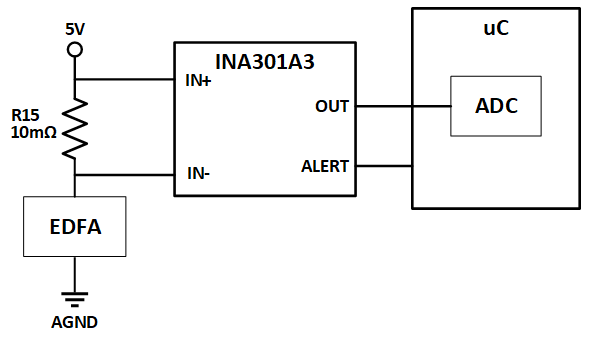
\includegraphics[width=0.75\textwidth]{./Figures/func_monitor.png}
\caption{Esquema del monitor de corriente}
\label{fig:funcMonitor}
\end{figure}



\subsection{Medición de tensión del amplificador}

Hacer una medición de la tensión de la línea es mucho mas sencillo que hacer una medición de la corriente, ya que esta se puede conectar directamente al ADC si previamente se la atenúa o amplifica (dependiendo del caso).

En este caso, como la tensión de alimentación del EDFA es 5 V y la tensión de referencia del ADC del microcontrolador es 3.3 V, se la debe atenuar. De esta forma la tensión máxima a medir se encuentra dentro del fondo de escala del ADC.

Considerando que se desea medir sobretensiones de por lo menos 1 V en la alimentación, se optó por atenuar la tensión del EDFA a la mitad, resultando en un fondo de escala de 6.6 V. En la figura \ref{fig:monTension} se puede ver el circuito implementado.

\begin{figure}[H]
\centering
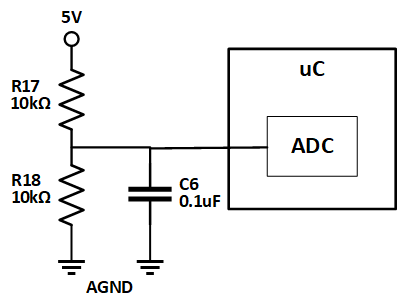
\includegraphics[width=0.5\textwidth]{./Figures/mon_tension.png}
\caption{Circuito del monitor de corriente}
\label{fig:monTension}
\end{figure}

\subsection{Pantalla LCD}

El modelo del módulo de la pantalla LCD utilizada en el trabajo es MSP2807 y es una solución integrada, es decir, cuenta con toda la electrónica necesaria para poder hacer uso de la pantalla en su totalidad. Para esto cuenta con dos circuitos integrados: el controlador del display de la pantalla (lo que permite dibujar en ella) y el controlador de la función táctil (lo que permite detectar cuando se la toca). Ambos chips tienen una interfaz SPI para ser controlados mas otras señales adicionales para funciones específicas.

\section{Arquitectura de software}

\subsection{Maquina de estados}

\subsection{Capa de abstracción del amplificador}


